Dos recintos bien mezclados de un taller contienen un aerosol trazador. Sus volúmenes constantes son \(V_1=50\) y \(V_2=100\,\mathrm{m^3}\). Circulan \(5\,\mathrm{m^3/min}\) en cada sentido entre ambos. Además, cada recinto recibe aire limpio del exterior y expulsa al exterior el mismo caudal: \(10\,\mathrm{m^3/min}\) el primero y \(20\,\mathrm{m^3/min}\) el segundo. Fuentes constantes añaden \(5\) y \(10\,\mathrm{mg/min}\), respectivamente.

Un limpiador sin intercambio neto de aire retira en el primer recinto una fracción \(k_1=0.10\,\mathrm{min}^{-1}\) de la cantidad de aerosol por unidad de tiempo. En el segundo, el coeficiente inicial es \(k_2=0\). No hay otras pérdidas. Los parámetros son sintéticos, y ambas concentraciones comienzan en \(0.20\,\mathrm{mg/m^3}\).

Formule los balances de cantidad y el sistema para las concentraciones \(c_1,c_2\). Determine si pueden representarse exactamente mediante una sola concentración común durante toda la evolución. Establezca qué condiciones sobre las fuentes y las tasas de eliminación por unidad de volumen harían válida esa reducción para cualquier concentración inicial común. Manteniendo los demás datos, determine qué valor de \(k_2\) la permitiría y escriba entonces la EDO para la concentración común.

\Needspace{9.17cm}
\begin{center}
\begin{minipage}{\linewidth}
\centering
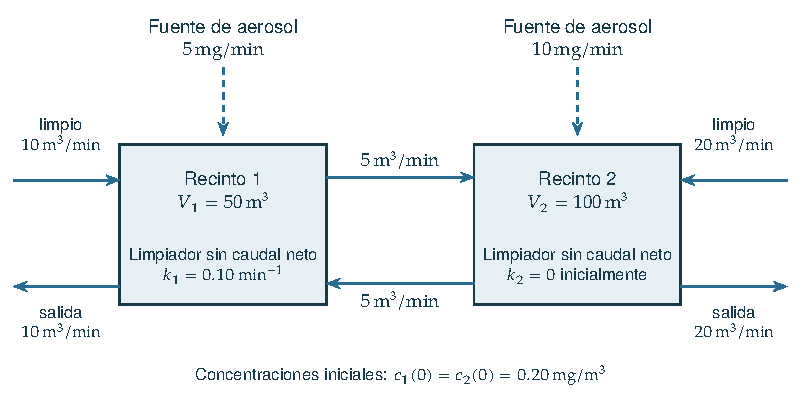
\includegraphics[width=15.18cm]{assets/M2-E0343-setup.pdf}\par
\smallskip{\small Ventilación, fuentes de aerosol y limpieza interna de los dos recintos.\par}
\end{minipage}
\end{center}
